\documentclass[twoside]{book}

% Packages required by doxygen
\usepackage{fixltx2e}
\usepackage{calc}
\usepackage{doxygen}
\usepackage[export]{adjustbox} % also loads graphicx
\usepackage{graphicx}
\usepackage[utf8]{inputenc}
\usepackage{makeidx}
\usepackage{multicol}
\usepackage{multirow}
\PassOptionsToPackage{warn}{textcomp}
\usepackage{textcomp}
\usepackage[nointegrals]{wasysym}
\usepackage[table]{xcolor}

% Font selection
\usepackage[T1]{fontenc}
\usepackage[scaled=.90]{helvet}
\usepackage{courier}
\usepackage{amssymb}
\usepackage{sectsty}
\renewcommand{\familydefault}{\sfdefault}
\allsectionsfont{%
  \fontseries{bc}\selectfont%
  \color{darkgray}%
}
\renewcommand{\DoxyLabelFont}{%
  \fontseries{bc}\selectfont%
  \color{darkgray}%
}
\newcommand{\+}{\discretionary{\mbox{\scriptsize$\hookleftarrow$}}{}{}}

% Page & text layout
\usepackage{geometry}
\geometry{%
  a4paper,%
  top=2.5cm,%
  bottom=2.5cm,%
  left=2.5cm,%
  right=2.5cm%
}
\tolerance=750
\hfuzz=15pt
\hbadness=750
\setlength{\emergencystretch}{15pt}
\setlength{\parindent}{0cm}
\setlength{\parskip}{3ex plus 2ex minus 2ex}
\makeatletter
\renewcommand{\paragraph}{%
  \@startsection{paragraph}{4}{0ex}{-1.0ex}{1.0ex}{%
    \normalfont\normalsize\bfseries\SS@parafont%
  }%
}
\renewcommand{\subparagraph}{%
  \@startsection{subparagraph}{5}{0ex}{-1.0ex}{1.0ex}{%
    \normalfont\normalsize\bfseries\SS@subparafont%
  }%
}
\makeatother

% Headers & footers
\usepackage{fancyhdr}
\pagestyle{fancyplain}
\fancyhead[LE]{\fancyplain{}{\bfseries\thepage}}
\fancyhead[CE]{\fancyplain{}{}}
\fancyhead[RE]{\fancyplain{}{\bfseries\leftmark}}
\fancyhead[LO]{\fancyplain{}{\bfseries\rightmark}}
\fancyhead[CO]{\fancyplain{}{}}
\fancyhead[RO]{\fancyplain{}{\bfseries\thepage}}
\fancyfoot[LE]{\fancyplain{}{}}
\fancyfoot[CE]{\fancyplain{}{}}
\fancyfoot[RE]{\fancyplain{}{\bfseries\scriptsize Generated by Doxygen }}
\fancyfoot[LO]{\fancyplain{}{\bfseries\scriptsize Generated by Doxygen }}
\fancyfoot[CO]{\fancyplain{}{}}
\fancyfoot[RO]{\fancyplain{}{}}
\renewcommand{\footrulewidth}{0.4pt}
\renewcommand{\chaptermark}[1]{%
  \markboth{#1}{}%
}
\renewcommand{\sectionmark}[1]{%
  \markright{\thesection\ #1}%
}

% Indices & bibliography
\usepackage{natbib}
\usepackage[titles]{tocloft}
\setcounter{tocdepth}{3}
\setcounter{secnumdepth}{5}
\makeindex

% Hyperlinks (required, but should be loaded last)
\usepackage{ifpdf}
\ifpdf
  \usepackage[pdftex,pagebackref=true]{hyperref}
\else
  \usepackage[ps2pdf,pagebackref=true]{hyperref}
\fi
\hypersetup{%
  colorlinks=true,%
  linkcolor=blue,%
  citecolor=blue,%
  unicode%
}

% Custom commands
\newcommand{\clearemptydoublepage}{%
  \newpage{\pagestyle{empty}\cleardoublepage}%
}

\usepackage{caption}
\captionsetup{labelsep=space,justification=centering,font={bf},singlelinecheck=off,skip=4pt,position=top}

%===== C O N T E N T S =====

\begin{document}

% Titlepage & ToC
\hypersetup{pageanchor=false,
             bookmarksnumbered=true,
             pdfencoding=unicode
            }
\pagenumbering{alph}
\begin{titlepage}
\vspace*{7cm}
\begin{center}%
{\Large animals }\\
\vspace*{1cm}
{\large Generated by Doxygen 1.8.13}\\
\end{center}
\end{titlepage}
\clearemptydoublepage
\pagenumbering{roman}
\tableofcontents
\clearemptydoublepage
\pagenumbering{arabic}
\hypersetup{pageanchor=true}

%--- Begin generated contents ---
\chapter{This is a small C++ example that shows the usage of inheritance, virtual methods and dynamic casts.}
\label{index}\hypertarget{index}{}\begin{DoxyAuthor}{Author}
Arno Wilhelm 
\end{DoxyAuthor}
\begin{DoxyVersion}{Version}
1.\+0 
\end{DoxyVersion}
\begin{DoxySince}{Since}
2018-\/05-\/29 
\end{DoxySince}

\chapter{Namespace Index}
\section{Namespace List}
Here is a list of all namespaces with brief descriptions\+:\begin{DoxyCompactList}
\item\contentsline{section}{\hyperlink{namespacestd}{std} }{\pageref{namespacestd}}{}
\end{DoxyCompactList}

\chapter{Hierarchical Index}
\section{Class Hierarchy}
This inheritance list is sorted roughly, but not completely, alphabetically\+:\begin{DoxyCompactList}
\item \contentsline{section}{Animal}{\pageref{classAnimal}}{}
\begin{DoxyCompactList}
\item \contentsline{section}{Cat}{\pageref{classCat}}{}
\item \contentsline{section}{Dog}{\pageref{classDog}}{}
\end{DoxyCompactList}
\end{DoxyCompactList}

\chapter{Class Index}
\section{Class List}
Here are the classes, structs, unions and interfaces with brief descriptions\+:\begin{DoxyCompactList}
\item\contentsline{section}{\hyperlink{classAnimal}{Animal} }{\pageref{classAnimal}}{}
\item\contentsline{section}{\hyperlink{classCat}{Cat} }{\pageref{classCat}}{}
\item\contentsline{section}{\hyperlink{classDog}{Dog} }{\pageref{classDog}}{}
\end{DoxyCompactList}

\chapter{File Index}
\section{File List}
Here is a list of all files with brief descriptions\+:\begin{DoxyCompactList}
\item\contentsline{section}{\hyperlink{animal_8h}{animal.\+h} }{\pageref{animal_8h}}{}
\item\contentsline{section}{\hyperlink{main_8cpp}{main.\+cpp} }{\pageref{main_8cpp}}{}
\end{DoxyCompactList}

\chapter{Namespace Documentation}
\hypertarget{namespacestd}{}\section{std Namespace Reference}
\label{namespacestd}\index{std@{std}}

\chapter{Class Documentation}
\hypertarget{classAnimal}{}\section{Animal Class Reference}
\label{classAnimal}\index{Animal@{Animal}}


{\ttfamily \#include $<$animal.\+h$>$}



Inheritance diagram for Animal\+:\nopagebreak
\begin{figure}[H]
\begin{center}
\leavevmode
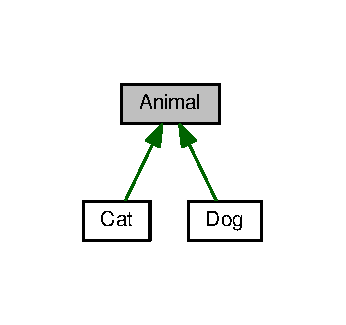
\includegraphics[width=166pt]{classAnimal__inherit__graph}
\end{center}
\end{figure}
\subsection*{Public Member Functions}
\begin{DoxyCompactItemize}
\item 
\hyperlink{classAnimal_a4ef4b49b9ed502193d9a1e447af9dca7}{Animal} (const string \&name)
\item 
const string \& \hyperlink{classAnimal_a9e5f35bbcafaddb2af949273d04a0055}{get\+Name} () const
\item 
virtual void \hyperlink{classAnimal_a1da8e52d19af5bd43a3755d9d5454598}{say\+Something} () const =0
\end{DoxyCompactItemize}
\subsection*{Private Attributes}
\begin{DoxyCompactItemize}
\item 
const string \hyperlink{classAnimal_af9bbbc58067910197fe5d7330e5cf09a}{name\+\_\+}
\end{DoxyCompactItemize}


\subsection{Detailed Description}
abstract base class of all derived animal classes.

\begin{DoxyAuthor}{Author}
Arno Wilhelm 
\end{DoxyAuthor}
\begin{DoxyVersion}{Version}
1.\+0 
\end{DoxyVersion}
\begin{DoxySince}{Since}
2018-\/05-\/29 
\end{DoxySince}


\subsection{Constructor \& Destructor Documentation}
\mbox{\Hypertarget{classAnimal_a4ef4b49b9ed502193d9a1e447af9dca7}\label{classAnimal_a4ef4b49b9ed502193d9a1e447af9dca7}} 
\index{Animal@{Animal}!Animal@{Animal}}
\index{Animal@{Animal}!Animal@{Animal}}
\subsubsection{\texorpdfstring{Animal()}{Animal()}}
{\footnotesize\ttfamily Animal\+::\+Animal (\begin{DoxyParamCaption}\item[{const string \&}]{name }\end{DoxyParamCaption})\hspace{0.3cm}{\ttfamily [inline]}}

Constructor


\begin{DoxyParams}{Parameters}
{\em name} & Name of the animal. \\
\hline
\end{DoxyParams}


\subsection{Member Function Documentation}
\mbox{\Hypertarget{classAnimal_a9e5f35bbcafaddb2af949273d04a0055}\label{classAnimal_a9e5f35bbcafaddb2af949273d04a0055}} 
\index{Animal@{Animal}!get\+Name@{get\+Name}}
\index{get\+Name@{get\+Name}!Animal@{Animal}}
\subsubsection{\texorpdfstring{get\+Name()}{getName()}}
{\footnotesize\ttfamily const string\& Animal\+::get\+Name (\begin{DoxyParamCaption}{ }\end{DoxyParamCaption}) const\hspace{0.3cm}{\ttfamily [inline]}}

Getter returns the name of the animal.

\begin{DoxyReturn}{Returns}
string Returns the name of the animal. 
\end{DoxyReturn}
\mbox{\Hypertarget{classAnimal_a1da8e52d19af5bd43a3755d9d5454598}\label{classAnimal_a1da8e52d19af5bd43a3755d9d5454598}} 
\index{Animal@{Animal}!say\+Something@{say\+Something}}
\index{say\+Something@{say\+Something}!Animal@{Animal}}
\subsubsection{\texorpdfstring{say\+Something()}{saySomething()}}
{\footnotesize\ttfamily virtual void Animal\+::say\+Something (\begin{DoxyParamCaption}{ }\end{DoxyParamCaption}) const\hspace{0.3cm}{\ttfamily [pure virtual]}}

Virtual interface method must be implemented by derived classes. Depending on the type of animal they give print out an animal specific sound. 

Implemented in \hyperlink{classCat_a2da2143abb847a8719e302614ccb8d2e}{Cat}, and \hyperlink{classDog_aa76235fa1a137f2fccf5138e5b92d0b3}{Dog}.



\subsection{Member Data Documentation}
\mbox{\Hypertarget{classAnimal_af9bbbc58067910197fe5d7330e5cf09a}\label{classAnimal_af9bbbc58067910197fe5d7330e5cf09a}} 
\index{Animal@{Animal}!name\+\_\+@{name\+\_\+}}
\index{name\+\_\+@{name\+\_\+}!Animal@{Animal}}
\subsubsection{\texorpdfstring{name\+\_\+}{name\_}}
{\footnotesize\ttfamily const string Animal\+::name\+\_\+\hspace{0.3cm}{\ttfamily [private]}}



The documentation for this class was generated from the following file\+:\begin{DoxyCompactItemize}
\item 
\hyperlink{animal_8h}{animal.\+h}\end{DoxyCompactItemize}

\hypertarget{classCat}{}\section{Cat Class Reference}
\label{classCat}\index{Cat@{Cat}}


{\ttfamily \#include $<$animal.\+h$>$}



Inheritance diagram for Cat\+:\nopagebreak
\begin{figure}[H]
\begin{center}
\leavevmode
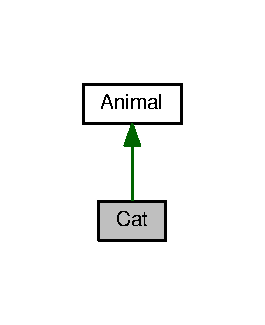
\includegraphics[width=127pt]{classCat__inherit__graph}
\end{center}
\end{figure}


Collaboration diagram for Cat\+:\nopagebreak
\begin{figure}[H]
\begin{center}
\leavevmode
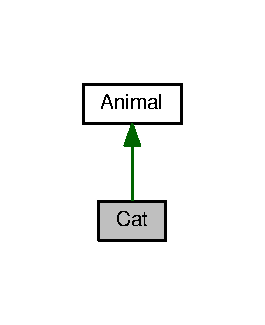
\includegraphics[width=127pt]{classCat__coll__graph}
\end{center}
\end{figure}
\subsection*{Public Member Functions}
\begin{DoxyCompactItemize}
\item 
\hyperlink{classCat_ae76478a80ba65c308a4efb251c3dc844}{Cat} (const string \&name)
\item 
void \hyperlink{classCat_a2da2143abb847a8719e302614ccb8d2e}{say\+Something} () const
\end{DoxyCompactItemize}
\subsection*{Additional Inherited Members}


\subsection{Detailed Description}
from class \hyperlink{classAnimal}{Animal}.

\begin{DoxyAuthor}{Author}
Arno Wilhelm 
\end{DoxyAuthor}
\begin{DoxyVersion}{Version}
1.\+0 
\end{DoxyVersion}
\begin{DoxySince}{Since}
2018-\/05-\/29 
\end{DoxySince}
\begin{DoxySeeAlso}{See also}
\hyperlink{classAnimal}{Animal} 
\end{DoxySeeAlso}


\subsection{Constructor \& Destructor Documentation}
\mbox{\Hypertarget{classCat_ae76478a80ba65c308a4efb251c3dc844}\label{classCat_ae76478a80ba65c308a4efb251c3dc844}} 
\index{Cat@{Cat}!Cat@{Cat}}
\index{Cat@{Cat}!Cat@{Cat}}
\subsubsection{\texorpdfstring{Cat()}{Cat()}}
{\footnotesize\ttfamily Cat\+::\+Cat (\begin{DoxyParamCaption}\item[{const string \&}]{name }\end{DoxyParamCaption})\hspace{0.3cm}{\ttfamily [inline]}}



\subsection{Member Function Documentation}
\mbox{\Hypertarget{classCat_a2da2143abb847a8719e302614ccb8d2e}\label{classCat_a2da2143abb847a8719e302614ccb8d2e}} 
\index{Cat@{Cat}!say\+Something@{say\+Something}}
\index{say\+Something@{say\+Something}!Cat@{Cat}}
\subsubsection{\texorpdfstring{say\+Something()}{saySomething()}}
{\footnotesize\ttfamily void Cat\+::say\+Something (\begin{DoxyParamCaption}{ }\end{DoxyParamCaption}) const\hspace{0.3cm}{\ttfamily [inline]}, {\ttfamily [virtual]}}

Implements the say\+Something method of base class \hyperlink{classAnimal}{Animal} and prints out a cat specific sound.

\begin{DoxySeeAlso}{See also}
\hyperlink{classAnimal_a1da8e52d19af5bd43a3755d9d5454598}{Animal\+::say\+Something} 
\end{DoxySeeAlso}


Implements \hyperlink{classAnimal_a1da8e52d19af5bd43a3755d9d5454598}{Animal}.



The documentation for this class was generated from the following file\+:\begin{DoxyCompactItemize}
\item 
\hyperlink{animal_8h}{animal.\+h}\end{DoxyCompactItemize}

\hypertarget{classDog}{}\section{Dog Class Reference}
\label{classDog}\index{Dog@{Dog}}


{\ttfamily \#include $<$animal.\+h$>$}



Inheritance diagram for Dog\+:\nopagebreak
\begin{figure}[H]
\begin{center}
\leavevmode
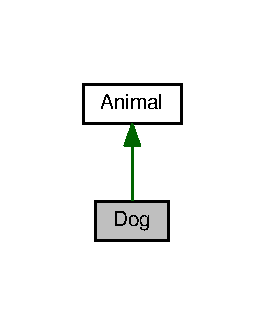
\includegraphics[width=127pt]{classDog__inherit__graph}
\end{center}
\end{figure}


Collaboration diagram for Dog\+:\nopagebreak
\begin{figure}[H]
\begin{center}
\leavevmode
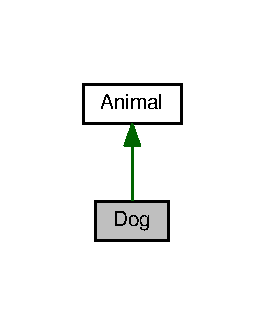
\includegraphics[width=127pt]{classDog__coll__graph}
\end{center}
\end{figure}
\subsection*{Public Member Functions}
\begin{DoxyCompactItemize}
\item 
\hyperlink{classDog_ad68949296d9449aa7d290e6f07d92787}{Dog} (const string \&name)
\item 
void \hyperlink{classDog_aa76235fa1a137f2fccf5138e5b92d0b3}{say\+Something} () const
\end{DoxyCompactItemize}
\subsection*{Additional Inherited Members}


\subsection{Detailed Description}
from class \hyperlink{classAnimal}{Animal}.

\begin{DoxyAuthor}{Author}
Arno Wilhelm 
\end{DoxyAuthor}
\begin{DoxyVersion}{Version}
1.\+0 
\end{DoxyVersion}
\begin{DoxySince}{Since}
2018-\/05-\/29 
\end{DoxySince}
\begin{DoxySeeAlso}{See also}
\hyperlink{classAnimal}{Animal} 
\end{DoxySeeAlso}


\subsection{Constructor \& Destructor Documentation}
\mbox{\Hypertarget{classDog_ad68949296d9449aa7d290e6f07d92787}\label{classDog_ad68949296d9449aa7d290e6f07d92787}} 
\index{Dog@{Dog}!Dog@{Dog}}
\index{Dog@{Dog}!Dog@{Dog}}
\subsubsection{\texorpdfstring{Dog()}{Dog()}}
{\footnotesize\ttfamily Dog\+::\+Dog (\begin{DoxyParamCaption}\item[{const string \&}]{name }\end{DoxyParamCaption})\hspace{0.3cm}{\ttfamily [inline]}}



\subsection{Member Function Documentation}
\mbox{\Hypertarget{classDog_aa76235fa1a137f2fccf5138e5b92d0b3}\label{classDog_aa76235fa1a137f2fccf5138e5b92d0b3}} 
\index{Dog@{Dog}!say\+Something@{say\+Something}}
\index{say\+Something@{say\+Something}!Dog@{Dog}}
\subsubsection{\texorpdfstring{say\+Something()}{saySomething()}}
{\footnotesize\ttfamily void Dog\+::say\+Something (\begin{DoxyParamCaption}{ }\end{DoxyParamCaption}) const\hspace{0.3cm}{\ttfamily [inline]}, {\ttfamily [virtual]}}

Implements the say\+Something method of base class \hyperlink{classAnimal}{Animal} and prints out a dog specific sound.

\begin{DoxySeeAlso}{See also}
\hyperlink{classAnimal_a1da8e52d19af5bd43a3755d9d5454598}{Animal\+::say\+Something} 
\end{DoxySeeAlso}


Implements \hyperlink{classAnimal_a1da8e52d19af5bd43a3755d9d5454598}{Animal}.



The documentation for this class was generated from the following file\+:\begin{DoxyCompactItemize}
\item 
\hyperlink{animal_8h}{animal.\+h}\end{DoxyCompactItemize}

\chapter{File Documentation}
\hypertarget{animal_8h}{}\section{animal.\+h File Reference}
\label{animal_8h}\index{animal.\+h@{animal.\+h}}
{\ttfamily \#include $<$string$>$}\newline
{\ttfamily \#include $<$iostream$>$}\newline
Include dependency graph for animal.\+h\+:\nopagebreak
\begin{figure}[H]
\begin{center}
\leavevmode
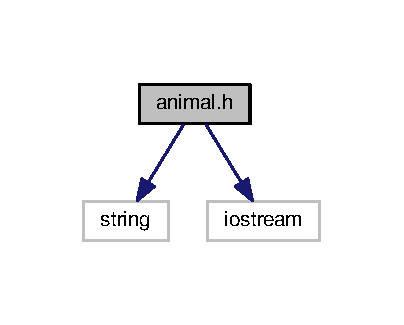
\includegraphics[width=194pt]{animal_8h__incl}
\end{center}
\end{figure}
This graph shows which files directly or indirectly include this file\+:\nopagebreak
\begin{figure}[H]
\begin{center}
\leavevmode
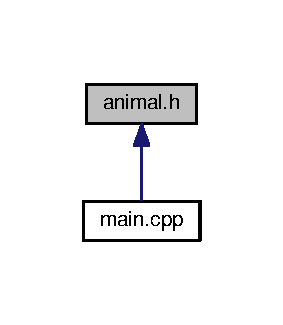
\includegraphics[width=136pt]{animal_8h__dep__incl}
\end{center}
\end{figure}
\subsection*{Classes}
\begin{DoxyCompactItemize}
\item 
class \hyperlink{classAnimal}{Animal}
\item 
class \hyperlink{classDog}{Dog}
\item 
class \hyperlink{classCat}{Cat}
\end{DoxyCompactItemize}
\subsection*{Namespaces}
\begin{DoxyCompactItemize}
\item 
 \hyperlink{namespacestd}{std}
\end{DoxyCompactItemize}

\hypertarget{main_8cpp}{}\section{main.\+cpp File Reference}
\label{main_8cpp}\index{main.\+cpp@{main.\+cpp}}
{\ttfamily \#include $<$iostream$>$}\newline
{\ttfamily \#include \char`\"{}animal.\+h\char`\"{}}\newline
Include dependency graph for main.\+cpp\+:\nopagebreak
\begin{figure}[H]
\begin{center}
\leavevmode
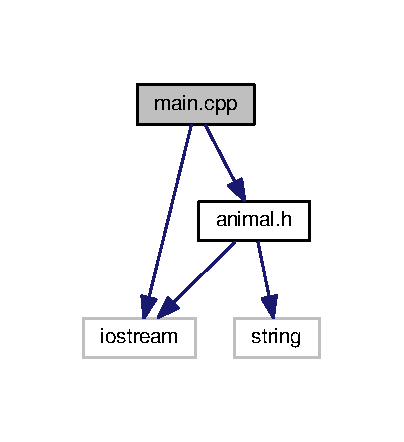
\includegraphics[width=194pt]{main_8cpp__incl}
\end{center}
\end{figure}
\subsection*{Functions}
\begin{DoxyCompactItemize}
\item 
int \hyperlink{main_8cpp_ae66f6b31b5ad750f1fe042a706a4e3d4}{main} ()
\end{DoxyCompactItemize}


\subsection{Function Documentation}
\mbox{\Hypertarget{main_8cpp_ae66f6b31b5ad750f1fe042a706a4e3d4}\label{main_8cpp_ae66f6b31b5ad750f1fe042a706a4e3d4}} 
\index{main.\+cpp@{main.\+cpp}!main@{main}}
\index{main@{main}!main.\+cpp@{main.\+cpp}}
\subsubsection{\texorpdfstring{main()}{main()}}
{\footnotesize\ttfamily int main (\begin{DoxyParamCaption}{ }\end{DoxyParamCaption})}


%--- End generated contents ---

% Index
\backmatter
\newpage
\phantomsection
\clearemptydoublepage
\addcontentsline{toc}{chapter}{Index}
\printindex

\end{document}
